\documentclass[a4paper,12pt]{article}
\usepackage{style}

\begin{document}

\begin{titlepage}
    \vspace*{7cm}
    
    \centering
    {\huge \bfseries Домашнее задание №1} \\[0.2cm]
    
    \hfill
    \begin{minipage}{0.4\textwidth}
        \begin{flushleft} \large
            Сахань В.С.
        \end{flushleft}
    \end{minipage}
    
    \vfill
    {\large \today}
\end{titlepage}

\section{Итерационные методы нелинейной оптимизации}

\subsection{Постановка задачи}
Требуется найти минимум функции $f(x,y) = \sin(x)\cdot\cos(y)+0,1(x^2+y^2)$ используя итерационный метод нелинейной оптимизации.

\subsection{Визуализация функции и ее линий уровня}
\begin{figure}[h!]
    \centering
    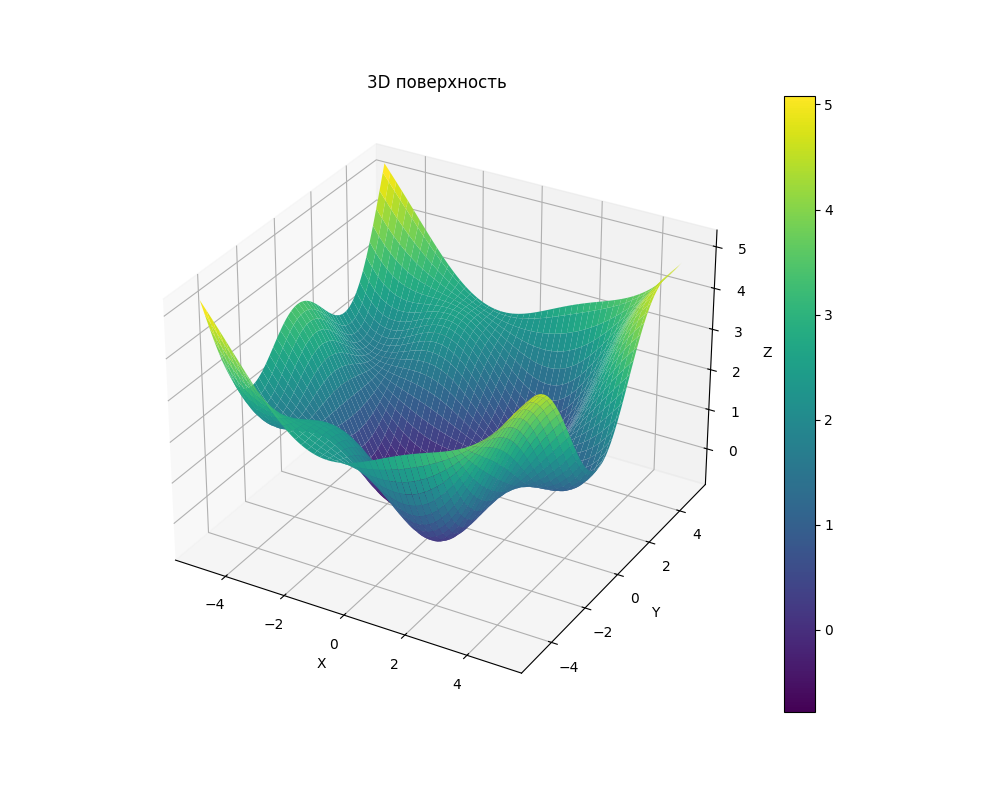
\includegraphics[width=1\textwidth]{imgs/surface.png} 
    \caption{Рельеф исследуемой функции}
    \label{fig:surface_plot}
\end{figure}

\begin{figure}[h!]
    \centering
    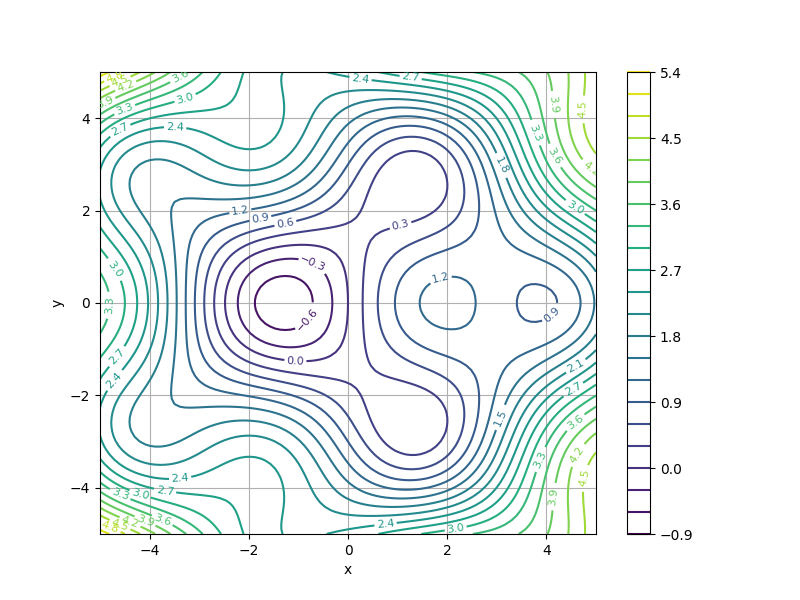
\includegraphics[width=1\textwidth]{imgs/level_lines.png} 
    \caption{Линии уровня исследуемой функции}
    \label{fig:level_lines_plot}
\end{figure}

\subsection{Рyчной расчет}

\subsubsection*{Итерация 1 (Минимизация по $x$)}
\[
\mathbf{x}^{(0)} = \begin{pmatrix} 2 \\ 1 \end{pmatrix}, \quad \mathbf{S}^{(0)} = \begin{pmatrix} -1 \\ 0 \end{pmatrix}
\]
\[
\mathbf{x}^{(1)} = \mathbf{x}^{(0)} + a \mathbf{S}^{(0)} = \begin{pmatrix} 2 - \alpha \\ 2 \end{pmatrix}
\]

Подставим в функцию $f(x, y) =  \sin(x)\cdot\cos(y)+0,1(x^2+y^2)$:
\[
\psi(\alpha) = \sin(2-\alpha)\cdot\cos(1)+0,1((2-\alpha)^2+1)
\]
\subsubsection*{Минимизация \psi(\alpha) методом Ньютона}

Для поиска локального минимума функции $\psi(\alpha)$ выберем начальное приближение $\alpha_1 = 2$. Шаг метода Ньютона:
\[
\alpha_{k+1} = \alpha_k - \frac{\psi'(\alpha_k)}{\psi''(\alpha_k)}
\]

Производные целевой функции:
\begin{align*}
    \psi'(\alpha) &= 0,2\cdot \alpha - \cos{(1)}\cdot\cos{(\alpha - 2)} - 0,4 \\
    \psi''(\alpha) &= \sin(\alpha - 2)\cdot\cos(1) + 0,2 
\end{align*}

Результаты итераций представлены в таблице:

\begin{center}
\begin{tabular}{|c|c|c|c|c|c|}
\hline
$k$ & $\alpha_k$ & $\psi(\alpha_k)$ & $\psi'(\alpha_k)$ & $\psi''(\alpha_k)$ & $\alpha_{k+1}$ \\ \hline
1 & 2.00000 & 0.10000 & -0.54030 & 0.20000 & 4.70151 \\ \hline
2 & 4.70151 & 0.59964 & 1.02912 & 0.43018 & 2.30918 \\ \hline
3 & 2.30918 & -0.05484 & -0.45285 & 0.36440 & 3.55189 \\ \hline
4 & 3.55189 & -0.19937 & 0.30017 & 0.74021 & 3.14638 \\ \hline
5 & 3.14638 & -0.26095 & 0.00678 & 0.69237 & 3.13658 \\ \hline
6 & 3.13658 & -0.26098 & 0.00001 & 0.69016 & 3.13656 \\ \hline
7 & 3.13656 & -0.26098 & 0.00000 & 0.69016 & 3.13656 \\ \hline
8 & 3.13656 & -0.26098 & 0.00000 & 0.69016 & 3.13656 \\ \hline
\end{tabular}
\end{center}

Оптимальный шаг $\alpha^* \approx 3.13656$.

Новая точка после первой полной итерации покоординатного спуска:
\[
\mathbf{x}^{(1)} = \mathbf{x}^{(0)} + \alpha^* \mathbf{S}^{(0)} = \begin{pmatrix} 2 \\ 1 \end{pmatrix} + 3.13656 \begin{pmatrix} -1 \\ 0 \end{pmatrix} = \begin{pmatrix} -1.13656 \\ 1 \end{pmatrix}
\]

\newpage
\subsubsection*{Итерация 2 (Минимизация по $y$)}
На предыдущем шаге была получена точка $x_1 = -1.13656$. Теперь фиксируем $x$ и минимизируем функцию по координате $y$:
\[
\mathbf{x}^{(2)} = \begin{pmatrix} -1.13656 \\ 1 \end{pmatrix}, \quad \mathbf{S}^{(1)} = \begin{pmatrix} 0 \\ -1 \end{pmatrix}
\]
\[
\mathbf{x}^{(2)} = \mathbf{x}^{(1)} + \alpha \mathbf{S}^{(1)} = \begin{pmatrix} -1.13656 \\ 1 - \alpha \end{pmatrix}
\]

\begin{equation}
    \psi(\alpha) = \sin(-1.13656) \cdot \cos(1-\alpha) + 0,1((-1.13656)^2 + (1-\alpha)^2)
\end{equation}

\subsubsection*{Минимизация \psi(\alpha) методом Ньютона}

Для нахождения локального минимума функции $\psi(\alpha)$ по направлению $\mathbf{S}^{(1)}$ выберем начальное приближение $\alpha_1 = 0,5$. Шаг метода Ньютона:
\[
\alpha_{k+1} = \alpha_k - \frac{\psi'(\alpha_k)}{\psi''(\alpha_k)}
\]

Производные:
\begin{align*}
    \psi'(\alpha) &= 0,2\cdot \alpha + 0,9072\cdot\sin(\alpha - 1) - 0,2 \\
    \psi''(\alpha) &= 0,9072\cdot\cos(\alpha - 1) + 0,2
\end{align*}


Результаты расчетов представлены в таблице:

\begin{center}
\begin{tabular}{|c|c|c|c|c|c|}
\hline
$k$ & $\alpha_k$ & $\psi(\alpha_k)$ & $\psi'(\alpha_k)$ & $\psi''(\alpha_k)$ & $\alpha_{k+1}$ \\ \hline
1 & 0.50000 & -0.64196 & -0.53493 & 0.99614 & 1.03701 \\ \hline
2 & 1.03701 & -0.77726 & 0.04097 & 1.10657 & 0.99999 \\ \hline
3 & 0.99999 & -0.77801 & -0.00002 & 1.10719 & 1.00000 \\ \hline
4 & 1.00000 & -0.77801 & 0.00000 & 1.10719 & 1.00000 \\ \hline
5 & 1.00000 & -0.77801 & 0.00000 & 1.10719 & 1.00000 \\ \hline
\end{tabular}
\end{center}

Оптимальный шаг по второй координате составил $\alpha^* \approx 1$. 

\subsubsection*{Итог итераций покоординатного спуска}
Последовательно выполнив минимизацию по $x$ и $y$, получаем точку:
\[
\mathbf{x}^{(2)} = \begin{pmatrix} -1.13656 \\ 0 \end{pmatrix}
\]
\\
Значение функции в начальной точке: $f(2, 1) \approx 0.991295$. \\
Значение функции после итераций: $f(-1.13656, 0) \approx -0.77801$. \\
Функция уменьшилась, что подтверждает корректность работы алгоритма.

\newpage
\subsubsection*{Визуализация метода}

\begin{figure}[h!]
    \centering
    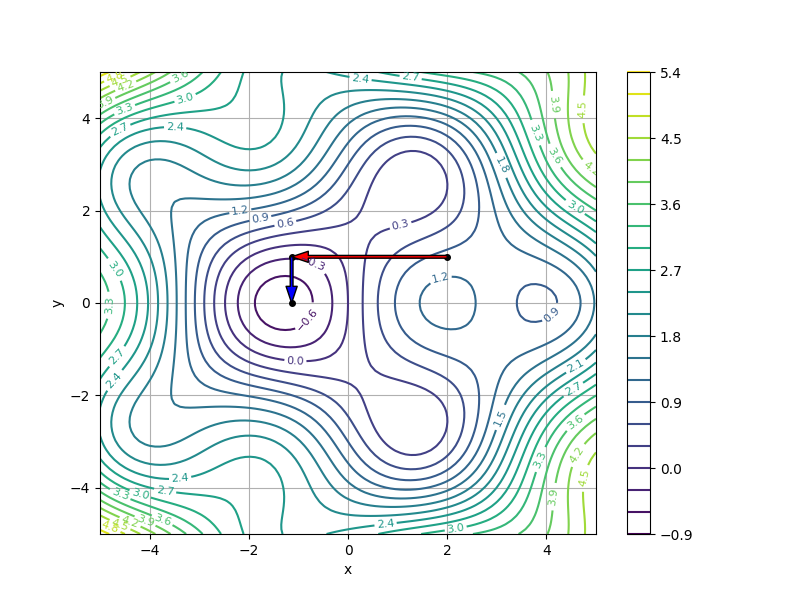
\includegraphics[width=1\textwidth]{imgs/vectors.png} 
    \caption{Визуализация метода}
    \label{fig:vectors}
\end{figure}

\newpage
\section{Задачи одномерной минимизации}

\subsection{Постановка задачи}
Требуется найти минимум унимодальной функции на отрезке [a,b] используя методы: дихотомии, золотого сечения, Фибоначчи, деления отрезка пополам и метода Ньютона.:

\begin{equation}
    f(x) = -\ln{x}-\ln{(1-x)}
\end{equation}
\\

Для нахождения минимума методом Ньютона вычислим первую и вторую производные:
\begin{align*}
    f'(x) &= \frac{-1 + 2x}{x(1 - x)}\\
    f''(x) &= \frac{2x^2 - 2x + 1}{(x - x^2)^2}
\end{align*}

\newpage
\subsection{Визуализация функции}
\begin{figure}[h!]
    \centering
    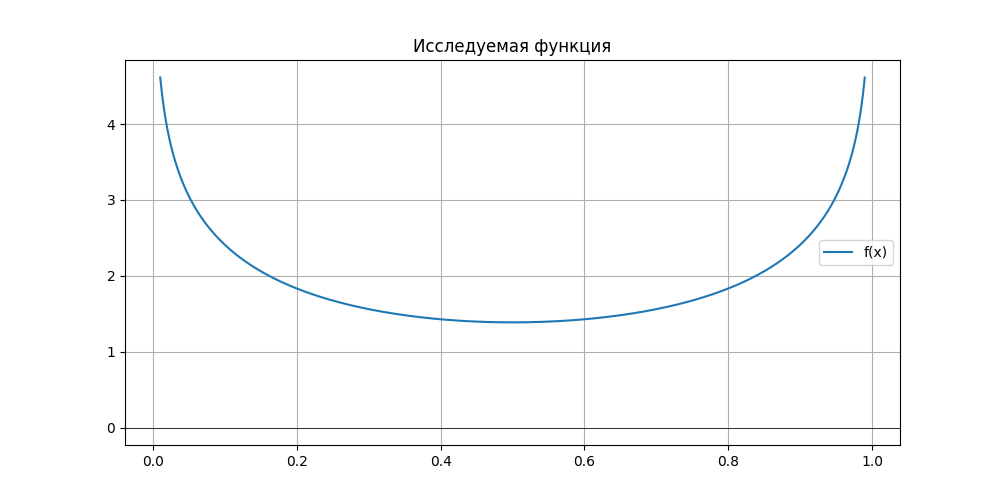
\includegraphics[width=1\textwidth]{imgs/func.png} 
    \caption{График исследуемой функции}
    \label{fig:func_plot}
\end{figure}

\subsubsection {Метод Ньютона в начальной точке 0,7}

\begin{center}
\begin{tabular}{|c|c|c|c|c|c|} \hline
k & x_k & f(x_k) & f'(x_k) & f''(x_k) & x_{k+1} \\ \hline
0 & 0.7000 & 1.5606 & 1.9048 & 13.1519 & 0.5552 \\ \hline
1 & 0.5552 & 1.3985 & 0.4468 & 8.2983 & 0.5013 \\ \hline
2 & 0.5013 & 1.3863 & 0.0106 & 8.0002 & 0.5000 \\ \hline
3 & 0.5000 & 1.3863 & 0.0000 & 8.0000 & 0.5000 \\ \hline
\end{tabular}
\end{center}
Минимум был достигнут за четыре итерации, $x^*=0,5$.

\begin{figure}[h!]
    \centering
    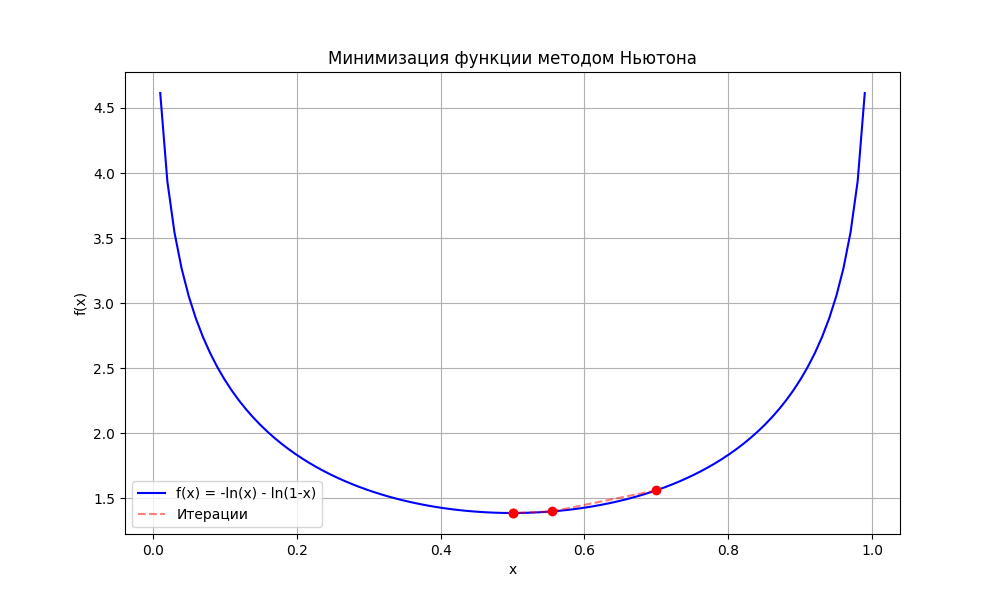
\includegraphics[width=1\textwidth]{imgs/newton.png} 
    \caption{Иллюстрация минимизации функции методом Ньютона}
    \label{fig:newton2}
\end{figure}

\newpage
\subsection {Метод Дихотомии на интервале (-1, 1), \varepsilon = 0.1}

\begin{center}
\begin{tabular}{|c|c|c|c|c|c|c|c|} \hline
k & a_k & b_k & l_k & x_1 & x_2 & f(x_1) & f(x_2) \\ \hline
0 & -1.0000 & 1.0000 & 2.0000 & -0.0100 & 0.0100 & 1 & 4.6152 \\ \hline
1 & -0.0100 & 1.0000 & 1.0100 & 0.4850 & 0.5050 & 1.3872 & 1.3864 \\ \hline
2 & 0.4850 & 1.0000 & 0.5150 & 0.7325 & 0.7525 & 1.6299 & 1.6807 \\ \hline
3 & 0.4850 & 0.7525 & 0.2675 & 0.6087 & 0.6287 & 1.4348 & 1.4549 \\ \hline
4 & 0.4900 & 0.6300 & & & & & \\ \hline
\end{tabular}
\end{center}

Алгоритм завершает работу, $x^*=(a + b )/ 2 = 0,56 $

\begin{figure}[h!]
    \centering
    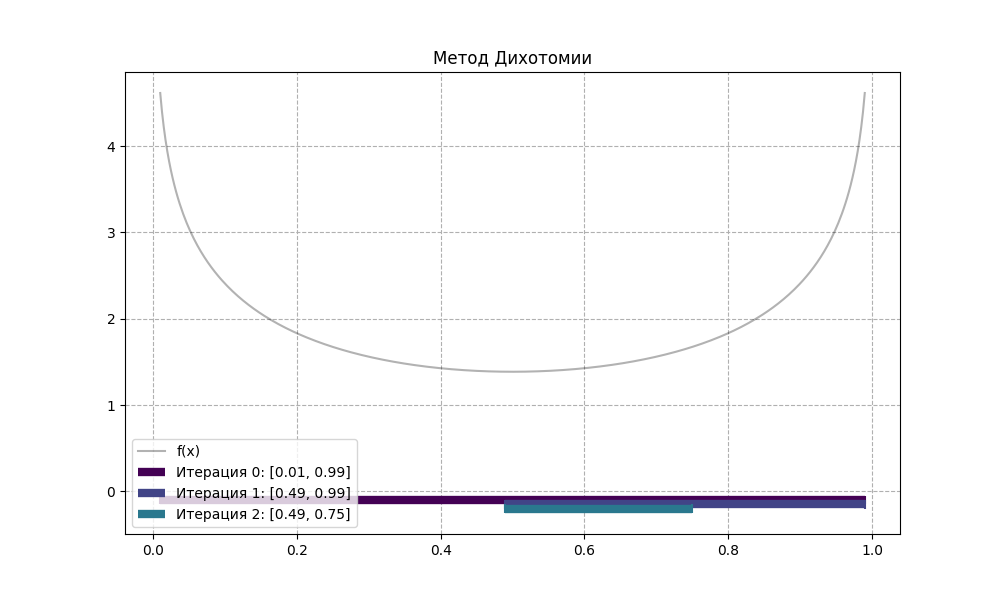
\includegraphics[width=1\textwidth]{imgs/dihotomy.png} 
    \caption{Иллюстрация метода Дихотомии}
    \label{fig:dihotomy}
\end{figure}

\newpage
\subsection{Метод золотого сечения на интервале (-1, 1), \varepsilon = 0.1}

\begin{center}
\begin{tabular}{|c|c|c|c|c|c|c|c|} \hline
k & a_k & b_k & l_k & x_1 & x_2 & f(x_1) & f(x_2) \\ \hline
0 & 0.01 &     0.99 &     0.98 &   0.3843 &   0.6157 &   1.4413 &   1.4413 \\ \hline
1 &   0.3843 &     0.99 &   0.6057 &   0.6157 &   0.7587 &   1.4413 &   1.6977 \\ \hline
2 &   0.3843 &   0.7587 &   0.3743 &   0.5273 &   0.6157 &   1.3893 &   1.4413 \\ \hline
3 &   0.3843 &   0.6157 &   0.2313 &   0.4727 &   0.5273 &   1.3893 &   1.3893 \\ \hline
4 &   0.4727 &   0.6157 &    0.143 &   0.5273 &   0.5611 &   1.3893 &   1.4013 \\ \hline
5 &   0.4727 &   0.56105 & & & & & \\ \hline
\end{tabular}
\end{center}

Алгоритм завершает работу, $x^*=(a + b )/ 2 = 0.5169 $

\begin{figure}[h!]
    \centering
    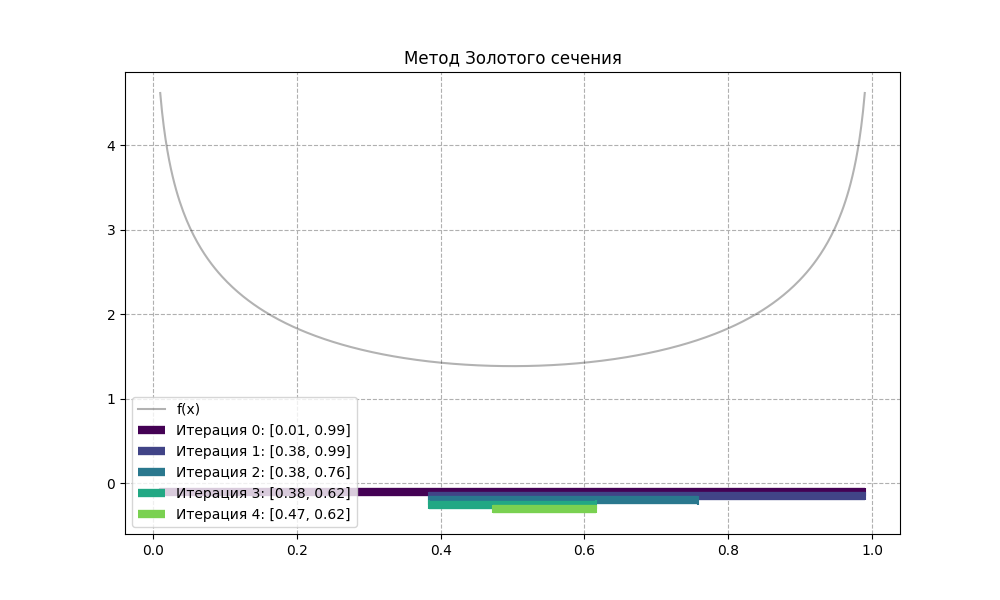
\includegraphics[width=1\textwidth]{imgs/golden_section.png} 
    \caption{Иллюстрация метода Золотого сечения}
    \label{fig:golden_raito}
\end{figure}

\newpage
\subsection{Метод Фибоначчи на интервале (-1, 1), \varepsilon = 0.1}
$F_n > \frac{b-a}{\varepsilon}= \frac{1-(-1)}{0,1}=20$ \\
Числа Фибоначчи: [1, 1, 2, 3, 5, 8, 13, 21] \\
Количество итераций $n = 7$
\begin{center}
\begin{tabular}{|c|c|c|c|c|c|c|c|} \hline
k & a_k & b_k & l_k & x_1 & x_2 & f(x_1) & f(x_2) \\ \hline
0 &     0.01 &     0.99 &     0.98 &   0.3869 &   0.6131 &   1.4388 &   1.4388 \\ \hline
1 &   0.3869 &     0.99 &   0.6031 &   0.6131 &   0.7638 &   1.4388 &   1.7127 \\ \hline
2 &   0.3869 &   0.7638 &   0.3769 &   0.5377 &   0.6131 &    1.392 &   1.4388 \\ \hline
3 &   0.3869 &   0.6131 &   0.2262 &   0.4623 &   0.5377 &    1.392 &    1.392 \\ \hline
4 &   0.4623 &   0.6131 &   0.1508 &   0.5377 &   0.5377 &    1.392 &    1.392 \\ \hline
5 &   0.5377 &   0.6131 &   0.0754 &   0.5377 &   0.6131 &    1.392 &   1.4388 \\ \hline
6 &  0.5377 & 0.61308 &   && & & \\ \hline
\end{tabular}
\end{center}

Последняя итерация, $x^*=0.5754

\begin{figure}[h!]
    \centering
    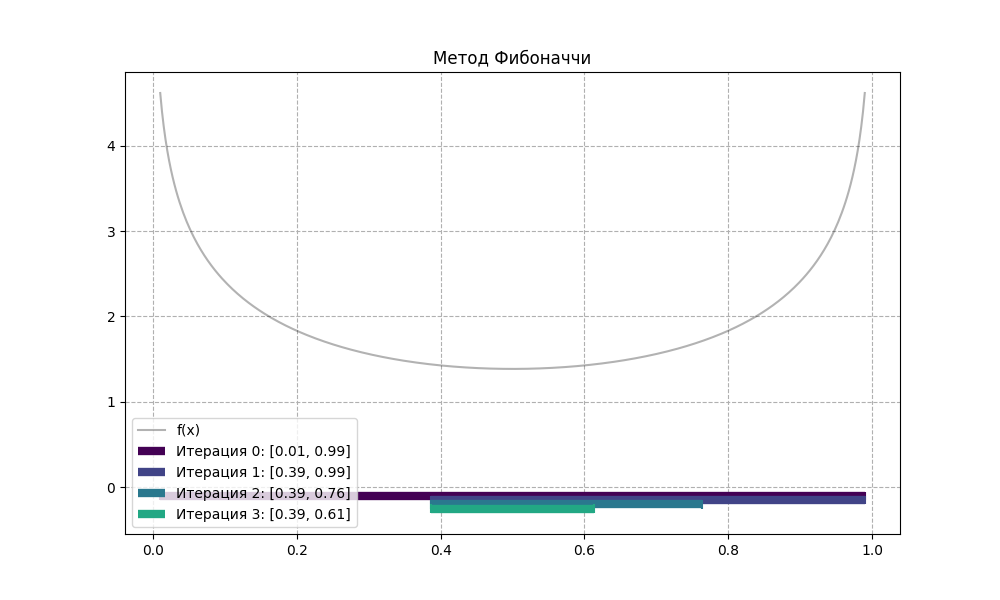
\includegraphics[width=1\textwidth]{imgs/fibonacci.png} 
    \caption{Иллюстрация метода Фибоначчи}
    \label{fig:fibonacchi}
\end{figure}

\newpage
\subsection{Метод Деления отрезка пополам (-1, 1), \varepsilon = 0.1}
\begin{center}
\begin{tabular}{|c|c|c|c|c|c|c|} \hline
k & a_k & b_k & l_k & mid & f'(mid) & f'(mid)>0 \\ \hline
0 &     0.01 &     0.99 &     0.98 &      0.5 &      0.0 &      Нет \\ \hline
1 &      0.5 &     0.99 &     0.49 &    0.745 &   2.5793 &       Да \\ \hline
2 &      0.5 &    0.745 &    0.245 &   0.6225 &   1.0426 &       Да \\ \hline
3 &      0.5 &   0.6225 &   0.1225 &   0.5613 &   0.4975 &       Да \\ \hline
4 & 0.5 & 0.56125 &&&& \\ \hline
\end{tabular}
\end{center}

$x^*=(a+b)/2= 0.5306$

\begin{figure}[h!]
    \centering
    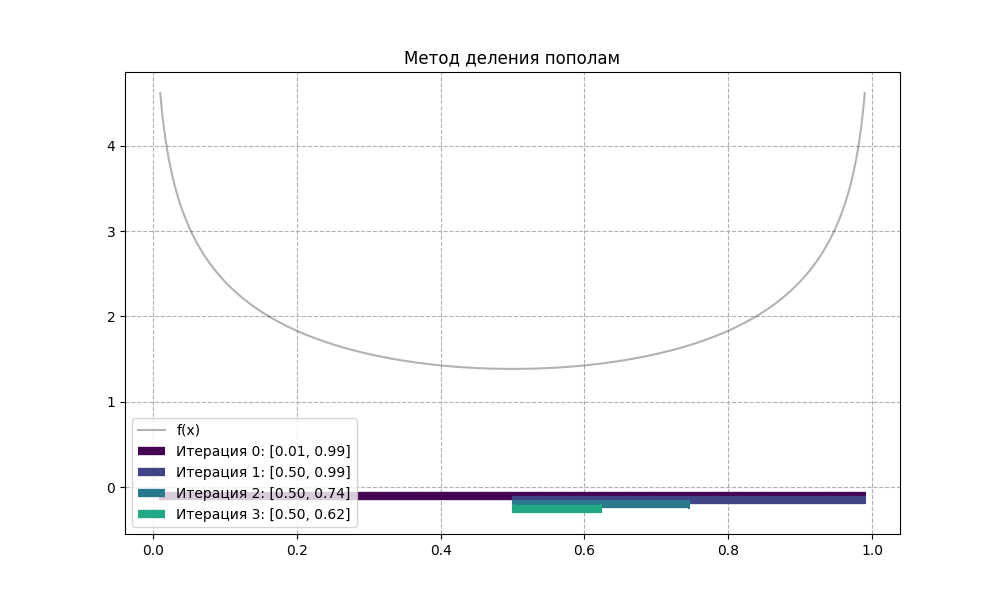
\includegraphics[width=1\textwidth]{imgs/halving.png} 
    \caption{Иллюстрация метода деления отрезка пополам}
    \label{fig:halving}
\end{figure}

\end{document}
